\lecture{2024-02-02}{}
\begin{example}
    $n$ guests attend a concert and leave their coats.
    At the end, each leaves with a random coat.
    Find the probability that none of them get their own coat back.
\end{example}
\begin{definition}[Derangement] \label{def:permutation:derangement}
    A permutation $\pi \in S_n$ is said to be a \emph{derangement} if \[
        \pi(i) \ne i \quad \text{for all } i \in [n].
    \] The number of derangements of $n$ objects is denoted $!n$.
\end{definition} 
\begin{example}
    The derangements of $[3]$ are $312$ and $231$.
\end{example}
We find the number of derangements on $[n]$.
Let $A_i = \set{\pi \in S_n \mid \pi(i) = i}$.
Then, \[
    A = \bigcup_i A_i = \set{\pi \in S_n \mid \exists i (\pi(i) = i)}.
\] Also note that $\abs{A_i} = (n-1)!$, $\abs{A_i \cap A_j} = (n-2)!$ and so
on (where $i \ne j$).
Thus by inclusion-exclusion, \begin{align*}
    \abs*[\bigg]{\bigcup_i A_i} &=
    \sum_{j=1}^{n} (-1)^{j-1} \sum_{S \in \binom{[n]}{j}}
        \abs*[\bigg]{\bigcap_{i \in S} A_i} \\
    &= \sum_{j=1}^{n} (-1)^{j-1} \binom{n}{j} (n-j)! \\
    &= n! \sum_{j=1}^{n} (-1)^{j-1} \frac{1}{j!}
    \intertext{and so the number of derangements is}
    !n &= n! - \abs*[\bigg]{\bigcup_i A_i} \\
    &= n! \sum_{j=0}^{n} (-1)^j \frac{1}{j!}.
\end{align*}
\begin{theorem*}[Derangement formula] \label{thm:derangement}
    The number of derangements of $n$ objects is \[
        !n = n! \sum_{j=0}^{n} \frac{(-1)^j}{j!}.
    \]
\end{theorem*}
This implies that $\frac{n!}{e}$ is a very good approximation for $!n$.

\subsection*{A more general formula}
Let $(P, \le)$ be a poset.
We say that $t$ \emph{covers} $s$, or that $s$ is covered by $t$, if $s < t$ and
there is no $u$ such that $s < u < t$.
The \emph{Hasse diagram} of $(P, \le)$ is the graph whose vertex set is $P$
and whose edges are the cover relations.
By convention, the smaller elements are drawn lower in the diagram.
\begin{example}
    The Hasse diagram of the poset $(2^{[3]}, \subseteq)$ is
    \begin{center}
        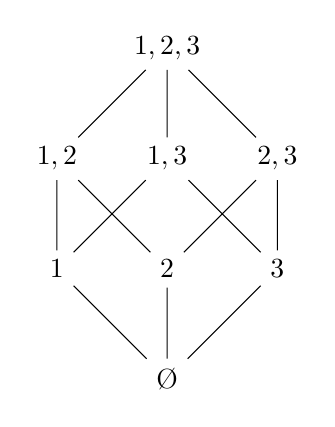
\begin{tikzpicture}[scale=1.4]
            \node (123) at (0, 0) {$\set{1, 2, 3}$};
            \node (12) at (-1, -1) {$\set{1, 2}$};
            \node (13) at (0, -1) {$\set{1, 3}$};
            \node (23) at (1, -1) {$\set{2, 3}$};
            \node (1) at (-1, -2) {$\set{1}$};
            \node (2) at (0, -2) {$\set{2}$};
            \node (3) at (1, -2) {$\set{3}$};
            \node (0) at (0, -3) {$\O$};
            \draw (123) -- (12)
                (123) -- (13)
                (123) -- (23)
                (12) -- (1)
                (12) -- (2)
                (13) -- (1)
                (13) -- (3)
                (23) -- (2)
                (23) -- (3)
                (1) -- (0)
                (2) -- (0)
                (3) -- (0);
        \end{tikzpicture}
    \end{center}
\end{example}

\begin{definition*}[Order ideal] \label{def:poset:order_ideal}
    An \emph{order ideal} of a poset $(P, \le)$ is a (non-empty) subset 
    $I \subseteq P$ such that if $t \in I$ and $s \le t$, then $s \in I$.
    The \emph{principal order ideal} generated by $t \in P$ is the set \[
        \downarrow t = \set{s \in P \mid s \le t}.
    \]
\end{definition*}
The principal order ideal generated by $t$ is an order ideal because of
transitivity, and is the minimal order ideal containing $t$.

\begin{definition*}[Möbius function] \label{def:poset:mobius_function}
    Let $(P, \le)$ be a poset for which every principal order ideal is
    finite.
    Then the \emph{Möbius function} $\mu\colon P \times P \to \Z$ is given by
    \begin{align*}
        \mu(s, s) &= 1, \\
        \mu(s, t) &= -\sum_{s \le u < t} \mu(s, u).
    \end{align*}
\end{definition*}
\begin{example}
    In the previous example of the poset $(2^{[3]}, \subseteq)$, we have
    \begin{align*}
        \mu(\O, \set{1}) &= -\smashoperator{\sum_{\O \le t < \set{1}}}
            \mu(\O, t) = -\mu(\O, \O) = -1, \\
        \mu(\O, \set{1, 2}) &= -\mu(\O, \O) - \mu(\O, \set{1}) - \mu(\O, \set{2}) \\
            &= -1 + 1 + 1 = 1
    \end{align*}
\end{example}

% \begin{lemma}
%     For each $t \in P$ and $s < t$, we have $\mu(s, t) = 0$.
%     In other words, for every $s \le t$, $\mu(s, t) = \delta_{s, t}$.
% \end{lemma}
% \begin{proof}
%     Since each principal order ideal is finite, we have that the set
%     $M_{s, t} = \set{u \in P \mid s \le u < t}$ is finite.
%     We induct on the size of this set.
%
%     For the base case $\#M_{s, t} = 1$, we have \[
%         \mu(s, t) = -\sum_{u \in M_{s, t}} \mu(s, u) = -\mu(s, s) = -1.
%     \]
% \end{proof}
\begin{theorem*}[Möbius inversion formula] \label{thm:mobius_inversion}
    Let $(P, \le)$ be a poset for which every principal order ideal is
    finite.
    Let $f, g\colon P \to \R$ be functions satisfying \begin{align*}
        g(t) &= \sum_{s \le t} f(s) \quad \text{for all } t \in P.
        \intertext{Then}
        f(t) &= \sum_{s \le t} \mu(s, t) g(s).
    \end{align*}
\end{theorem*}
\begin{proof}
    We have \begin{align*}
        \sum_{s \le t} \mu(s, t) g(s)
        &= \sum_{s \le t} \mu(s, t) \sum_{u \le s} f(u) \\
        &= \sum_{u \le t} \sum_{u \le s \le t} \mu(s, t) f(u) \\
        &= \sum_{u \le t} f(u) \sum_{u \le s \le t} \mu(s, t) \\
        &= \sum_{u \le t} f(u) \delta_{u, t}
    \end{align*}
    where $\delta_{u, t}$ is the Kronecker delta.
    Why is the last step true?
    If $u = t$, then \[
        \sum_{u \le s \le t} \mu(s, t) = \mu(t, t) = 1.
    \] Otherwise,
    \begin{align*}
        \sum_{u \le s \le t} \mu(s, t)
        &= \sum_{u \le s < t} \mu(s, t) + \mu(t, t) \\
        &= 1 - \mu(u, t).
    \end{align*}
\end{proof}
